%!TEX root = dissertacao.tex
\section{TEMPLATES}
\label{sec:templates}

\textit{Templates} de autômatos celulares são uma generalização de suas tabelas de transição de estado, capazes de representar famílias de regras. Os templates foram criados por de Oliveira e Verardo (\citeyear{deOliveira2014}) e implementados como um algoritmo na linguagem do software \textit{Wolfram Mathematica} \cite{woframMathematica10}, atualmente disponíveis na biblioteca \textit{open source CATemplates} \cite{CATemplates} no GitHub.

Formalmente, um \textit{template} é uma $n$-tupla formada por $k^{2r+1}$ itens, e cada item $i$ representa uma função $g_i(x_0,x_1,\dots,x_{k^{2r+1}-1})$. As variáveis $x_i$ podem assumir qualquer estado entre 0 e $k-1$, o que implica que, no caso binário, $x_i$ pode assumir os valores 0 e 1. Pode-se limitar os valores possíveis de $x_i$ através da notação $x_i \in C$, onde $C$ é um conjunto representando os possíveis valores de $x_i$; note-se, entretanto, que essa notação só tem sentido prático para ACs com quantidade de estados $k>2$.

Exemplificando, dado um template $T_1 = (1,1,1,1,1-x_1,x_2,x_1,0)$, ele representará todas as regras que tenham na posição 0 (sempre da direita para a esquerda) o estado 0, nas posições 4, 5, 6 e 7 o estado 1, nas posições 1 e 2 qualquer estado no intervalo $[0,k-1]$, e na posição 3 o estado complementar ao valor da posição 1. Perceba-se que o tamanho da $n$-tupla é $k^{2r+1}$, acarretando que no template $T_1$ os únicos valores inteiros possíveis para $k$ e $r$ são 2 e 1 respectivamente. Portanto $T_1$ representará um subespaço dos ACs elementares.

Deste modo o template $T_1$ representa o conjunto de autômatos celulares elementares $\{(1,1,1,1,1,0,0,0),(1,1,1,1,0,0,1,0),(1,1,1,1,1,1,0,0),(1,1,1,1,0,1,1,0)\}$, ou em suas formas decimais, o conjunto de regras $\{248,242,252,246\}$.

Cada template tem um número de substituições máximo igual a $k^m$, sendo $m$ o número de variáveis livres. O maior template possível de uma família de ACs é o \textit{template base}, em que todas as variáveis são livres, e que representa todas as regras do espaço em questão. O menor é o \textit{template constante}, em que não há variáveis livres, e representa, portanto, apenas uma regra. A $8$-tupla mostrada na Eq. \eqref{eq:templateConstante} representa um template constante que corresponde à regra elementar 30.  
\begin{equation}
(0,0,0,1,1,1,1,0)
\label{eq:templateConstante}
\end{equation}

Já a $8$-tupla, apresentada na Eq. \eqref{eq:templateBase}, representa um template base que está associado a todas as 256 regras do espaço elementar já que, para $m = 8$, temos $2^m = 256 $.
\begin{equation}
(x_7,x_6,x_5,x_4,x_3,x_2,x_1,x_0)
\label{eq:templateBase}
\end{equation}

É importante enfatizar que nem sempre o número de substituições é igual a $k^m$. Isto ocorre pois algumas substituições podem originar tabelas de transições inválidas. O template $(1,1,1,1,1,x_0+x_1,x_1,x_0)$, por exemplo, não pode apresentar as substituições $x_0=1$ e $x_1=1$ ao mesmo tempo, pois isso faz com que $x_0 + x_1 \notin [0, k-1]$, invalidando assim essa substituição para $k=2$.

A representação de famílias de autômatos celulares através de templates possibilita a utilização de templates para problemas já bem conhecidos da área de ACs. Um exemplo de problema que pode se beneficiar dos templates é o problema da paridade.

Para o problema de paridade, nesse projeto, considera-se um AC binário, unidimensional e com condição de contorno periódica. Se uma configuração inicial contiver um número ímpar de estados com valor 1, o AC deve convergir para uma configuração global onde toda as células estejam preenchidas com 1, caso contrário, ele deve convergir para todos os estados com o valor 0. Há um problema nessa definição para  reticulado de tamanho par, pois uma configuração inicial com todas as células apresentando o estado $1$ teriam que convergir para uma configuração com todos os estados apresentando o valor $0$. Entretanto, o problema define que uma configuração preenchida apenas por $1$s assim deve permanecer. Devido a isso, pode-se dizer que as regras que solucionam o problema de paridade em ACs são \textit{perfeitas} se eles resolverem o problema de paridade em qualquer configuração inicial arbitrária para ACs de tamanho ímpar \cite{Betel2013}. Conforme Betel, de Oliveira e Flocchini (\citeyear{Betel2013}) nos lembram, duas condições devem ser satisfeitas em relação ao problema de paridade. A primeira é que, se $f$ é a regra local que resolve o problema de paridade, então $f(0, \dots, 0) = 0$ e $f(1, \dots, 1) = 1$. A segunda é que, para uma regra preservar a configuração de paridade, ela deve apresentar número par de transições ativas (quais, sejam, as que imponham uma troca do bit de saída); em outras palavras, toda aplicação da regra deve levar a uma nova configuração com a mesma paridade.

A Figura \ref{fig:parity-rule} ilustra o desenvolvimento espaço-temporal da regra BFO \cite{Betel2013} que resolve o problema de paridade para o raio 4. Nessa imagem o desenvolvimento temporal à esquerda contém, em sua configuração inicial, um número par de estados igual a 1 e, na evolução temporal ilustrada à direita, um número ímpar de estados igual a 1.

\begin{figure}[h!]
\center
\subfigure[Configuração inicial com número ímpar de 1s]{
\includegraphics[width=3.7cm]{regra-1-par.pdf}}
\qquad
\subfigure[Configuração inicial com número par de 1s]{
\includegraphics[width=3.7cm]{regra-1-impar.pdf}}
\caption{Evolução espaço-temporal da regra BFO, que resolve o problema de paridade para raio 4 \cite{Betel2013}.}
\label{fig:parity-rule}
\end{figure}

O estudo do problema da paridade é interessante pois ajuda a compreender o impacto das interações locais nas soluções globais. Especificamente, entender a influência que o tamanho da vizinhança em autômatos celulares apresenta na computabilidade pode apresentar consequências úteis tanto para ACs, como para a compreensão de sistemas emergentes complexos em geral.

Estudos feitos sobre o problema de paridade já levaram ao conhecimento de que o problema não tem solução perfeita para ACs elementares e de raio 2. Todavia já foi descoberta uma regra perfeita que soluciona o problema de paridade para raio 4. Em relação aos ACs de raio 3, ainda não foi encontrada solução perfeita e há evidências empíricas desfavoráveis a uma solução para esse raio \cite{Betel2013}.

Betel, de Oliveira e Flocchini (\citeyear{Betel2013}), buscando verificar se o problema da paridade em ACs de raio 2 apresentam alguma regra que solucione o problema para qualquer configuração inicial, encontraram de forma analítica como as transições de estado de supostas regras que resolvessem o problema de paridade deveriam ser. 

Para representar como as transições de estado deveriam ser, foram utilizados grafos de De Bruijn. Grafos de De Bruijn são grafos, propostos de forma independentes por De Bruijn (\citeyear{Bruijn946combinatorial}) e \citeonline{Good1946normal}, cujos nós são sequências de símbolos de algum alfabeto e cujas arestas indicam as sequências em que se cruzarão \cite{weisstein2015deBruijn}. Em AC, esse tipo de grafo direcionado representa em cada uma de suas arestas uma vizinhança possível, e o valor associado às arestas será o resultado da transição, dada à vizinhança representada pela aresta. A Figura \ref{fig:grafosDeBruijnSample} ilustra dois grafos de De Bruijn, sendo que o primeiro pode ser utilizado para ilustrar todas as vizinhanças possíveis dos autômatos celulares elementares.
\begin{figure}[h!]
\centering
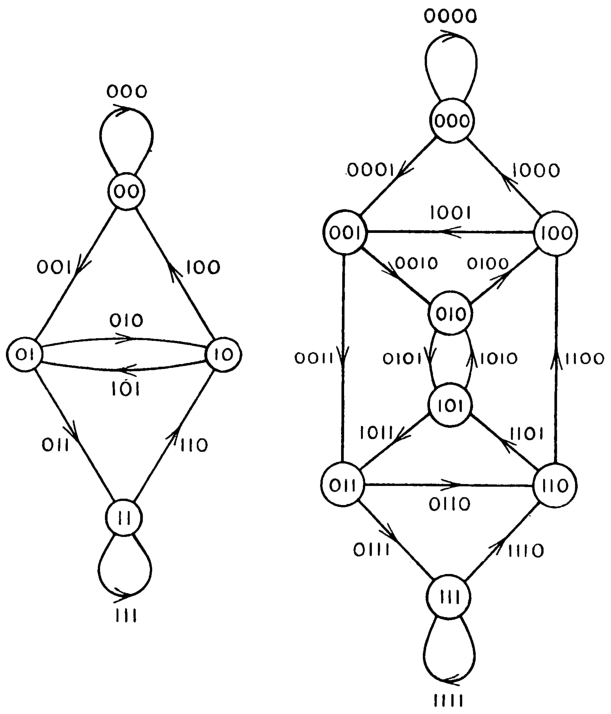
\includegraphics[width=0.3\textwidth]{fig_graphDeBruijn.pdf}
\caption{Exemplo de grafo de De Bruijn \cite{Good1946normal}}
\label{fig:grafosDeBruijnSample}
\end{figure}

Com isso, utilizando grafos de De Bruijn, foram definidas quais variáveis deveriam ser valores constantes, quais deveriam ser livres, e quais deveriam apresentar interdependência. Com essas definições foram encontrados dois conjuntos de ACs. Os grafos ilustrados na Figura \ref{fig:grafosDeBruijn} e na Figura \ref{fig:grafosDeBruijn2} são os grafos desenvolvidos por Betel, de Oliveira e Flocchini (\citeyear{Betel2013}).
\begin{figure}[h!]
\centering
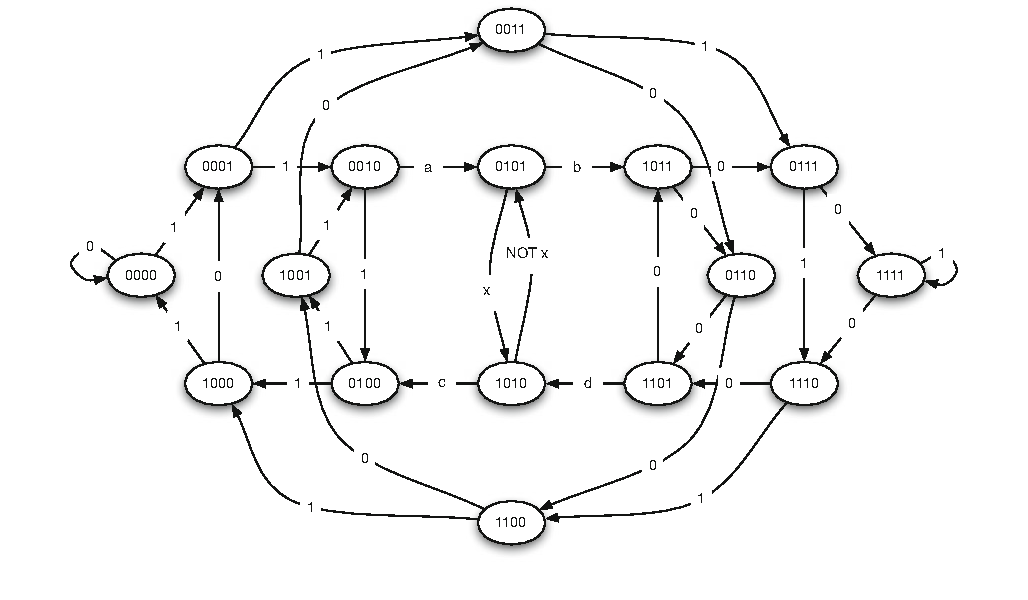
\includegraphics[width=0.7\textwidth]{grafo1.pdf}
\caption{Grafo de De Bruijn representando regras que possivelmente solucionassem o problema de paridade \cite{Betel2013}.}
\label{fig:grafosDeBruijn}
\end{figure}

\begin{figure}[h!]
\centering
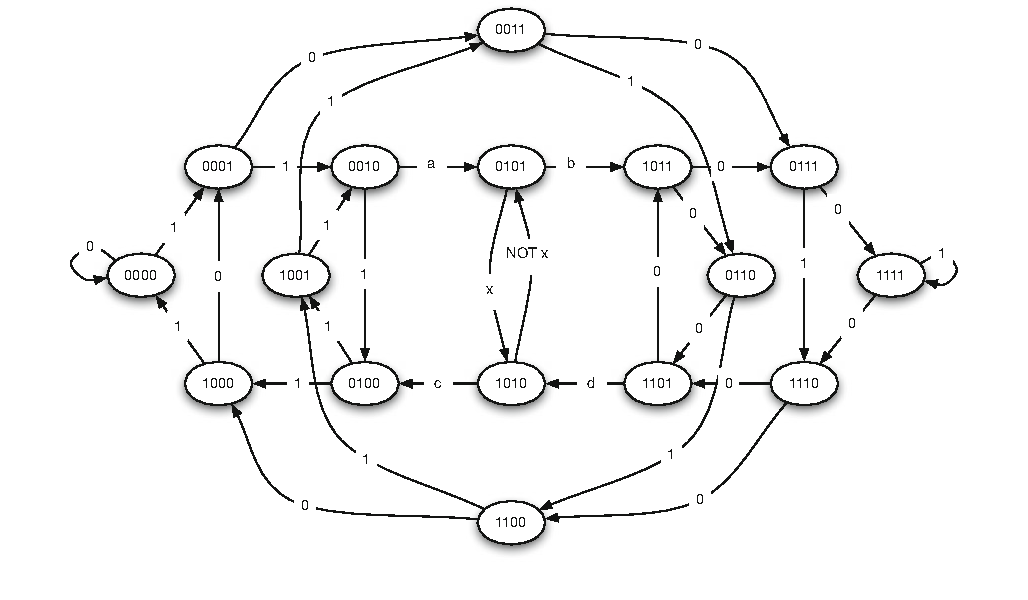
\includegraphics[width=0.7\textwidth]{grafo2.pdf}
\caption{Outro grafo de De Bruijn representando regras adicionais que possivelmente solucionassem o problema de paridade \cite{Betel2013}.}
\label{fig:grafosDeBruijn2}
\end{figure}

Ambos os grafos apresentam arestas contendo as variáveis livres $a, b, c, d \text{ e } x$ e uma interdependência, em que uma transição de estado deve ter o valor oposto à variável $x$. A única diferença entre os dois grafos está nas arestas contendo variáveis estáticas.

Ao utilizar os grafos de De Bruijn, fixando algumas transições de estado, a família de ACs em que se procurava as regras que solucionariam o problema de paridade foi restringida para apenas 64 regras. Ao se restringir o espaço de busca, antes composto por $2^{32}$ regras, as regras puderam ser estudadas em mais detalhes até que falhassem. Entretanto, conforme mostrado em \cite{Verardo2014}, a representação desse espaço de 64 regras pode ser equivalentemente representado por meio de \textit{templates}. O template da Eq. \eqref{eq:templateParidade1} representa o mesmo espaço que a Figura \ref{fig:grafosDeBruijn}, e o template da Eq. \eqref{eq:templateParidade2} é equivalente à Figura \ref{fig:grafosDeBruijn2}. Ambos os templates referem-se a raio $r=2$ e 2 estados.
\begin{equation}
\left(0,1,1,1,1,x_{26},0,1,1,1,1-x_{10},x_{20},0,0,1,0,1,0,1,0,x_{11},x_{10},0,0,1,0,x_5,0,1,0,0,1\right)
\label{eq:templateParidade1}
\end{equation}
\begin{equation}
\left(0,1,1,0,1,x_{26},1,0,1,1,1-x_{10},x_{20},0,1,1,0,1,0,1,1,x_{11},x_{10},0,0,1,0,x_5,0,0,0,0,1\right)
\label{eq:templateParidade2}
\end{equation}


\newpage\newpage
\subsection{Expansão de Templates}
Expansão é o processo pelo qual se obtêm todas as tabelas de transição $R_k$ associadas a um template $T$.
A operação de expansão foi apresentada por \citeonline{Verardo2014} e foi descrita em mais detalhes da seguinte maneira:

\begin{equation}
E(T)=R_k
\end{equation}

A operação de expansão pode ser dividida em dois passos: processamento e pós-processamento. O primeiro consiste em efetuar todas as $k^m$ substituições de variáveis possíveis. Considere como exemplo o template $T_1 = (1,1,1,1,1-x_1,x_2,x_1,0)$, o primeiro passo do processo de expansão consiste em encontrar as tabelas $k$-árias resultantes das combinações possíveis das substituições de $x_1$ e $x_2$, conforme pode ser melhor visualizado na Tabela \ref{tab:expansionProcess}.
\begin{table}[h!]
\centering
\caption{Processo de expansão.}
	\begin{tabular}{cccc}
    \toprule
	$i$ & $x_2$ & $x_1$ & Tabela $k$-ária resultante \\
    \midrule
	0	&	0	&	0	&	(1,1,1,1,1,0,0,0)	\\
	1	&	0	&	1	&	(1,1,1,1,1,1,0,0)	\\
	2	&	1	&	0	&	(1,1,1,1,0,0,1,0)	\\
	3	&	1	&	1	&	(1,1,1,1,0,1,1,0)	\\
    \bottomrule
	\end{tabular}
\label{tab:expansionProcess}
\end{table}

O pós-processamento da operação de expansão pode variar de acordo com o template. No template que representa as regras conservativas de paridade, por exemplo, o pós-processamento consiste em aplicar a operação $mod$ $2$ em cada um dos campos das tabelas $k$-ária. Em templates com restrições de variáveis, é no pós-processamento que se eliminam as tabelas $k$-árias incompatíveis com as restrições. Mas na maioria dos casos o pós-processamento não é necessário, ou ele consiste apenas em eliminar as tabelas $k$-árias inválidas. No caso do template $T_1$ acima todas as tabelas resultantes são válidas e nenhum pós-processamento se faz necessário; mas nem sempre isso ocorre. No template $T_2 = (1,1,1,1,1,x_0+x_1,x_1,x_0)$, por exemplo, a substituição $x_0 = 1$ e $x_1 = 1$ resulta numa tabela $k$-ária inválida, pois a posição $2$ resultaria em um estado com valor fora do intervalo $[0,k-1]$, para $k=2$. A Tabela \ref{tab:invalideExpansion} evidencia melhor essa substituição inválida.
\begin{table}[h!]
\centering
\caption{Processo de expansão}
	\begin{tabular}{cccc}
    \toprule
	$i$ & $x_1$ & $x_0$ & tabela $k$-ária resultante \\
    \midrule
	0	&	0	&	0	&	(1,1,1,1,1,0,0,0)	\\
	1	&	0	&	1	&	(1,1,1,1,1,1,0,1)	\\
	2	&	1	&	0	&	(1,1,1,1,1,1,1,0)	\\
	3	&	1	&	1	&	(1,1,1,1,1,2,1,1)	\\
    \bottomrule
   	\end{tabular}
\label{tab:invalideExpansion}
\end{table}

Conforme mostrado na Tabela \ref{tab:invalideExpansion}, para o template $T_2$ listar apenas regras válidas é necessário aplicar um pós-processamento que filtre as tabelas $k$-árias inválidas, no caso, a gerada pela expansão de $i = 3$. 

Um outro exemplo de template que resulta em substituições inválidas são os templates que utilizam a notação de restrição por conjuntos. Considere o template $T_3 = (2,2,2,2,2,2,2,2,x_0\in \{0,1\})$ da família de $k=3$ e $r=0{,}5$, sendo que raio $0{,}5$ define uma vizinhança com apenas dois campos. A substituição obtida para $i = 2$ (conforme a Tabela \ref{tab:invalideExpansion2}) seria inválida pois nesse caso $x_0 = 2 \notin \{0,1\}$, sendo assim necessário que o pós-processamento desconsidere essa expansão gerada.
\begin{table}[h!]
\centering
\caption{Processo de expansão}
	\begin{tabular}{cccc}
    \toprule
	$i$ & $x_0$ & tabela $k$-ária resultante \\
    \midrule
	0	&	0	&	(2,2,2,2,2,2,2,2,0)	\\
	1	&	1	&	(2,2,2,2,2,2,2,2,1)	\\
	2	&	2	&	(2,2,2,2,2,2,2,2,2)	\\
    \bottomrule
	\end{tabular}
\label{tab:invalideExpansion2}
\end{table}

A existência de regras inválidas possibilita templates que representem um conjunto de regras diferentes de $k^m$. Essa possibilidade é bastante útil para os templates de regras conservativas, regras conservativas de paridade e regras confinadas, que representam um número de regras diferente de $k^m$. Deste modo, toda vez que se gera um template, também é necessário informar que tipo de pós-processamento será necessário utilizar na hora da expansão. A Tabela \ref{tab:posProcessamento} mostra os pós-processamentos necessários para as principais funções geradoras de templates do \textit{CATemplates}:
\begin{table}[h!]
\centering
\caption{Pós-processamento necessário por templates}
	\begin{tabular}{ll}
    \toprule
	Template & Pós-processamento \\
    \midrule
	Template de regras confinadas 				& Filtrar regras com restrições inválidas	\\
	Template de conservabilidade de estados		& Filtrar regras inválidas						\\
	Template de conservabilidade de paridade 	& Aplicar $mod$ $2$ e filtrar regras inválidas	\\
	Template de totalidade e semi-totalidade 	& Nenhum pós-processamento necessário 				\\
	Templates de simetria		 				& Nenhum pós-processamento necessário 				\\
    \bottomrule
	\end{tabular}
\label{tab:posProcessamento}
\end{table}

Note-se que a $i$-ésima substituição, $i \in [0,k^m-1]$, sempre representa apenas uma substituição possível para as variáveis livres de um template. Isso ocorre pois $i$ é a representação decimal da conversão $k$-ária das concatenações dos valores das variáveis livres em ordem decrescente. Exemplificando, considere o templates $T_4 = (2,2,2,2,2,2,2,x_1\in \{0,1\},x_0)$ para $k=3$. O valor de $i=5$ será convertido pelo processo de expansão obtendo-se assim o seu equivalente na base ternária $(1,2)$ e então cada um dos dígitos é atribuído a uma variável, resultando assim no conjunto de substituições ${x_1=1,x_0=2}$.

A forma com que o valor de $i$ representa apenas uma expansão possibilita se obter a $i$-ésima expansão de um template. Essa propriedade é relevante devido ao fato de a expansão ser uma operação potencialmente custosa, e a possibilidade de ser realizar a $i$-ésima expansão de um template facilita e permite o paralelismo.

\newpage\newpage
\subsection{Intersecção de Templates}
Intersecção é o processo pelo qual, de dois templates $T_1$ e $T_2$, obtêm-se o template $T_3$ que representa o conjunto $R_k$. O conjunto $R_k$ representa todas as regras pertencentes aos dois templates recebidos como parâmetro. É necessário que os dois templates recebidos como parâmetro pertençam ao mesmo espaço. A operação de intersecção foi descrita por \citeonline{Verardo2014} e mostrada em mais detalhes da seguinte maneira:

\begin{equation}
I(T_1,T_2)=T_3 \Leftrightarrow E(T_3) = E(T_1) \cap E(T_2)
\end{equation}

A operação de intersecção, assim como a de expansão, também é efetuada em duas etapas. Na primeira etapa igualam-se os dois templates e assim se obtêm um sistema de equações. Esse sistema de equações é então passado como argumento para a função $Solve$, nativa da \textit{Wolfram Language} \cite{woframMathematica10}, para ser resolvido. A função $Solve$ retorna então os relacionamentos entre as variáveis, que ao serem aplicados aos templates recebidos, retorna dois templates equivalentes, bastando escolher um que será o template de intersecção. No caso dos templates não apresentarem intersecção, a função $Solve$ nada retornará.

Para melhor compreensão, considere os templates $T_1 = (x_7,x_3,1-x_4,x_4,x_3,x_2,2,x_0)$ e $T_2 = (x_7,1,x_5,0,x_3,x_2,2,2)$, ambos com $r=0{,}5$ e $k=3$. Esse templates serão transformados em um sistema de equações como demonstrado na Eq. \eqref{eq:interseccao}.

\begin{equation}
\left\{\begin{matrix}
x_7   & = & x_7 \\ 
x_3   & = & 1 \\ 
1-x_4 & = & x_5    \\ 
x_4   & = & 0    \\ 
x_3   & = & x_3    \\ 
x_2   & = & x_2   \\ 
2     & = & 2   \\ 
x_0   & = & 2
\end{matrix}\right.
\label{eq:interseccao}
\end{equation}

Esse sistema de equações é passado então como argumento para a função $Solve$ que, por sua vez, retorna um conjunto solução $S$, neste exemplo, $S = \{x_0 = 2, x_3 = 1, x_4 = 0, x_5 = 1 - x_4, x_6 = 0\}$. O conjunto $S$ é aplicado como um conjunto de substituições sobre os dois templates recebidos como parâmetro que, em caso de templates sem restrição de variáveis, sempre retorna o mesmo template. No exemplo, após aplicada as substituições do conjunto de soluções $S$, obtêm-se como resultado o template $T_3 = (x_7, 1, 1, 0, 1, x_2, 2, 2)$.

A segunda etapa do algoritmo é aplicada apenas para templates com alguma restrição de variável. Essa etapa consiste em extrair as expressões que estabelecem as restrições, e através delas obter um segundo sistema de equações. A solução desse sistema pode ser vazia, expressando assim que os templates não tem intersecção, ou pode indicar os valores que as variáveis com restrição podem assumir.

Para exemplificar essa segunda etapa, considerem-se os templates $T_{r1} = (x_7 \in \{0,1,2\},x_3,1-x_4,x_4,x_3,x_2 \in \{1,2\},2,x_0)$ e $T_{r2} = (x_7 \in \{0,1\},1,x_5,0,x_3,x_2 \in \{1\},2,2)$. A primeira etapa ocorre normalmente, entretanto, quando as substituições do conjunto $S$ forem aplicadas nos templates recebidos, não serão mais obtidos templates iguais, quais sejam, $\{(x_7 \in \{0,1,2\}, 1, 1, 0, 1, x_2 \in \{1,2\}, 2, 2), (x_7 \in \{0,1\}, 1, 1, 0, 1, x_2 \in \{1\}, 2, 2)\}$. Na sequência o algoritmo faz a extração das expressões de restrição de variáveis e obtêm o conjunto $\{x_7 \in \{0,1\}, x_2 \in \{1,2\}, x_2 \in \{1\} \}$. Esse conjunto é então convertido para o sistema de equações representadas pela Eq. \eqref{eq:interseccaoRestrita}.

\begin{equation}
\left\{\begin{matrix}
x_7	  = 0 	& \vee &	x_7	=	1 & \vee &	x_7	= 2	\\ 
x_7   = 0 	& \vee &	x_7	=	1					\\ 
x_2   = 1 	& \vee &	x_2	=	2					\\ 
x_2	  =	1											\\ 
\end{matrix}\right.
\label{eq:interseccaoRestrita}
\end{equation}

Esse sistema de equações é então passado como argumento para a função $Solve$, que retorna seu conjunto solução. Por fim o algoritmo usa o conjunto solução obtido para remover as restrições da variável $x_2$, transformando-a no valor $1$, e restringir a variável $x_7$ apenas ao conjunto $\{0,1\}$. O template de intersecção gerado por todo esse processo é representado pela Eq. \eqref{eq:templateIntescecao}.

\begin{equation}
T_{r3} = (x_7 \in \{0,1\}, x_3, 1-x_4, x_4, x_3, 1, 2, x_0)
\label{eq:templateIntescecao}
\end{equation}

Observe-se no exemplo que o template $T_{r2}$ também poderia ser representado substituindo a variável $x_2$ e seu conjunto de restrição $\{1\}$ apenas pelo valor constante $1$, como mostrado a seguir: $T_{r2} = (x_7 \in \{0,1\}, 1, x_5, 0, x_3, 1, 2, 2)$. Esse tipo de mudança é recomendado pois variáveis a mais acarretam em mais processamento.

Note-se ainda que, no caso binário ($k = 2$), a notação de restrição nunca é necessária, visto que ela terá apenas um valor factível, tornando preferível que essa variável e sua restrição sejam substituídas por um valor constante, ou a variável poderá assumir qualquer estado, sendo assim, por definição, uma variável livre.